\documentclass[slidestop,compress,mathserif]{beamer}
\usetheme{Frankfurt}
\usecolortheme{seagull}
\definecolor{links}{HTML}{2A1B81}
\hypersetup{colorlinks,linkcolor=,urlcolor=links}

% Load packages
\usepackage{alltt}
\usepackage{verbatim}
\usepackage{geometry}
\usepackage{graphicx}
\usepackage{amssymb}
\usepackage{amsmath}
\usepackage{epstopdf}
\usepackage{feynmp}
\usepackage{hyperref}

%\usepackage{pgfpages}
%\pgfpagesuselayout{4 on 1}[letterpaper,landscape,border shrink=5mm]

\DeclareGraphicsRule{.tif}{png}{.png}{`convert #1 `dirname #1`/`basename #1 .tif`.png}


% Title 
% Note: [short title]{long title}, [short author(s) name]{long author(s) name}
\title{LaTeX Basics}
\subtitle{}
\author{Viktor Dmitriyev} 
\institute{Adapted from Mini Course on LaTeX by \href{https://github.com/OpenIntroOrg/mini-course-materials}{David Diez}}

\date{}

\begin{document}
\definecolor{highlight}{rgb}{.7,.1,.1}
\definecolor{command}{rgb}{.1,.1,.9}
\definecolor{comment}{rgb}{1,0,0}
\definecolor{braces}{rgb}{0,0.5,0}
\newenvironment{act}[1]{{\color{command}#1}}{}


\frame{ \titlepage }

\begin{frame}
  \frametitle{Outline}
  \begin{itemize}
  \item Intro to LaTeX interface
  \item Working with text
  \item Tabbing and tables
  \item Figures
%  \item Math and equations
  \end{itemize}
\end{frame}

\part{}

\section[Getting started]{Getting started}
\subsection[Getting started]{Getting started}

\begin{frame} \frametitle{Installing LaTeX}
	
	{\bf Windows Installation. } Download proTeXt, which can be found on {\color{highlight}http://www.tug.org/protext/}\footnote{Another option: {\color{highlight}http://www.winshell.de/}. (Winshell and MikTeX)}. LaTeX can be accessed via TeXnicCenter, which is included in this installation. \\
	
	{\bf Mac Installation. } Download MacTeX, which can be found on {\color{highlight}http://www.tug.org/mactex/}. LaTeX can then be accessed via the program TeXShop, which is included in this installation. \\
	\vspace{0.5cm}

\end{frame}

\begin{frame} \frametitle{Installing LaTeX}
	
	\begin{itemize}
		\item Be careful that the distributive with LaTeX are very big. Use instead your own disk copy.
		\item Despite interfaces for Mac, Windows, and Linux are different, the same LaTeX ``code'' must works under all operating systems.
		\item There are many tools available to edit LaTeX files (actually any text editor can do that). But it order to make things easier here we are going to use TeXStudio ({\color{highlight}http://www.texstudio.org/}).
	\end{itemize}
	
\end{frame}


\begin{frame} \frametitle{Opening TeXStudio}
	Download and install TeXStudio ({\color{highlight}http://www.texstudio.org/}) on your PC in case it is not installed. Than navigate to directory that contains 'TeXStudio' and start it.

	\begin{center}
		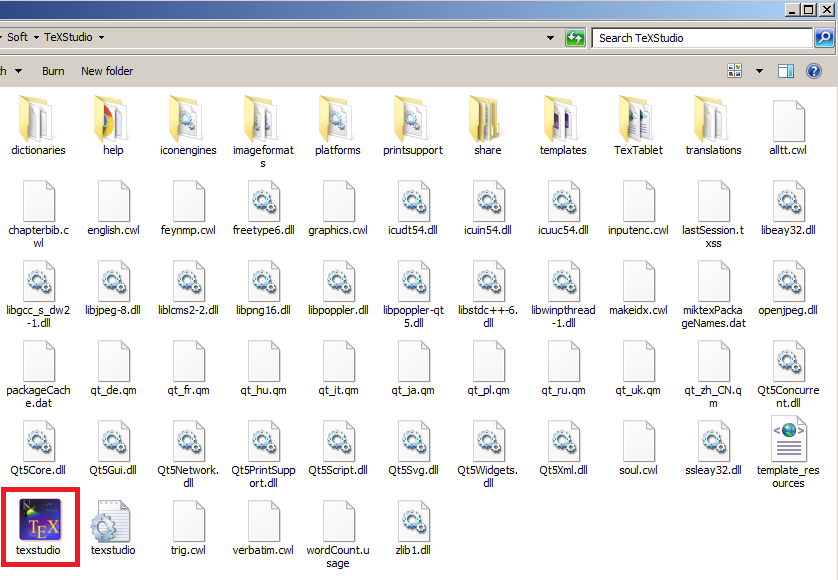
\includegraphics[height=1.7in]{basicsOfLatex/gettingStarted/texstudioFolder}
	\end{center}
\end{frame}


\begin{frame} \frametitle{Changing Interface Language of TexStudio}
	After installation TexStudio will use \textbf{standard} language of operating systems for user interface. To change language you need to navigate to proper panel and select the one you prefer:
	
	\vspace{0.5cm}
	
	\tiny{
		\textbf{English}: \textit{Option $\,\to\,$ Configure TeXstudio $\,\to\,$ General $\,\to\,$ Language}\\
		\textbf{German}:  \textit{Optionen $\,\to\,$ TeXstudio konfigurieren $\,\to\,$ Allgemein $\,\to\,$ Sprache}\\
	}
	
	\begin{center}
		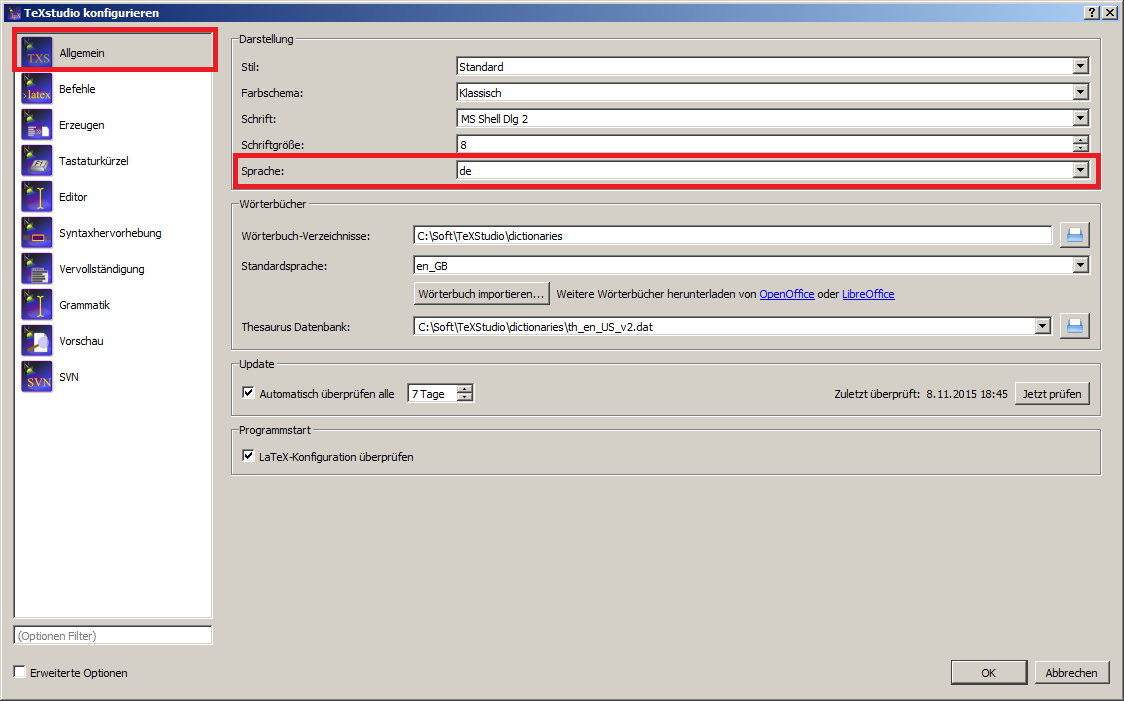
\includegraphics[height=1.7in]{basicsOfLatex/gettingStarted/texstudioLanguage}
	\end{center}
	
\end{frame}

\begin{frame} \frametitle{Creating a basic document}
	
	In order to start working with LaTeX you will need template of document. You can use given one (usually conferences or book has their own LaTeX templates), you standard one or create your own template.\\
	
	\vspace{0.5cm}
		
	{\bf Open a file.}  Use {\color{highlight}File $>$ New} or \texttt{\color{highlight}Ctrl+N}  to open a new document if one isn't already open. \\

	\vspace{0.5cm}

	{\bf Templates}. Use {\color{highlight} File $>$ New From Template}. \\
	\begin{center}
		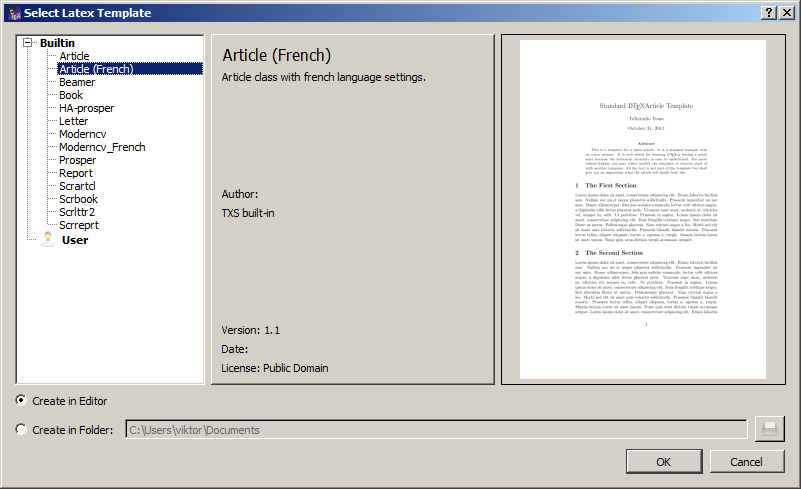
\includegraphics[height=0.95in]{basicsOfLatex/gettingStarted/texstudioTemplate}
	\end{center}
\end{frame}

\begin{frame} \frametitle{Creating a basic document}
Update the \texttt{\color{command}$\backslash$title}, \texttt{\color{command}$\backslash$author}, and then type a sentence above the last line, i.e. type right above \texttt{\color{command}$\backslash$end}{\color{braces}\{}document{\color{braces}\}}. Create a folder on the desktop and then save this file into that folder.
	\begin{center}
		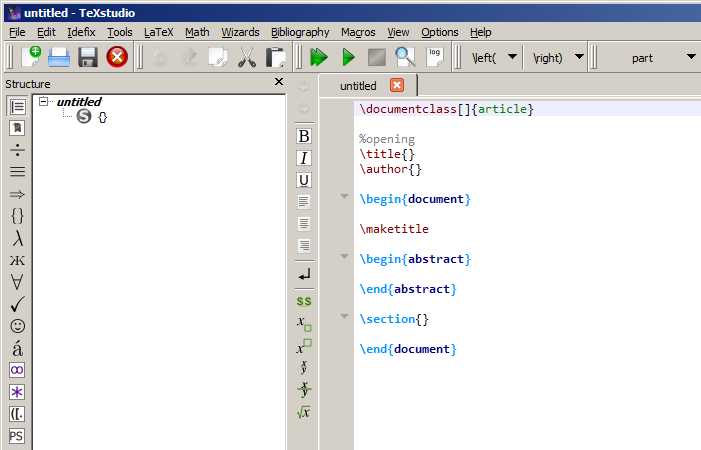
\includegraphics[height=2.0in]{basicsOfLatex/gettingStarted/texstudioFirstDocument}
	\end{center}
\end{frame}

\begin{frame} \frametitle{Typesetting / Compiling}
Different tools use different shortcuts to translate LaTeX file into PDF. Hit \texttt{\color{highlight}F5} or click the green {\color{highlight}Play} button at the top panel. After typesetting, double-click on the PDF page to magnify. Try triple-clicking... and quadruple-clicking.
\begin{center}
	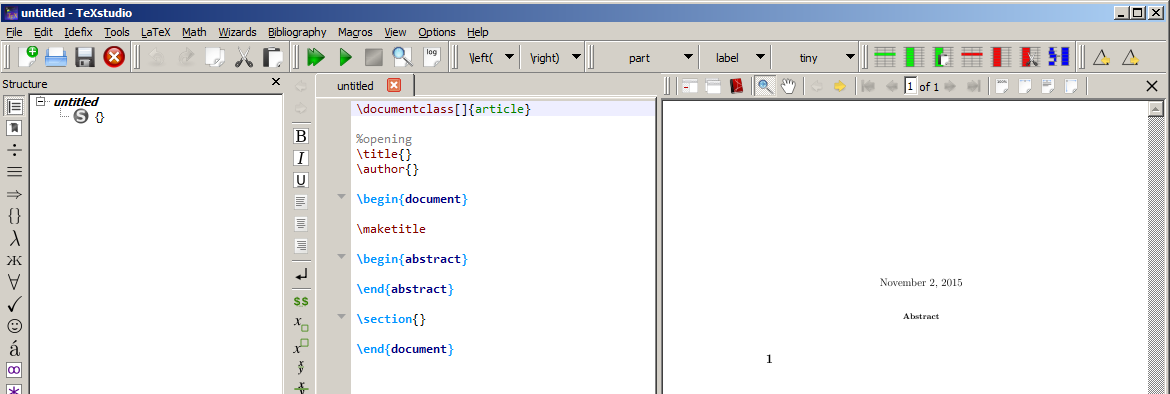
\includegraphics[height=2.0in]{basicsOfLatex/gettingStarted/texstudiofirstOutput}
\end{center}
\end{frame}

\begin{frame} \frametitle{Extra files}
Compilation creates a bunch of other files.
\begin{center}
	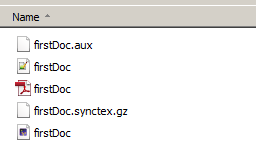
\includegraphics[height=1.0in]{basicsOfLatex/gettingStarted/texstudioExtraFiles}
\end{center}

While each of these files has a purpose, only one file -- in addition to the original LaTeX file -- is of interest: the PDF. As more methods of LaTeX are used, this list of LaTeX output files might grow... but again, they (except the .tex and .pdf files) can just be ignored for the vast majority of LaTeX use.
\end{frame}

\begin{frame} \frametitle{Console}
When the code was typeset, two windows popped up. The {\color{highlight}console} tells you what LaTeX is doing when it runs through the document. If there is an error (or just something LaTeX doesn't like), the console will tell you. If the error is critical, LaTeX will stop compiling:
	\begin{center}
		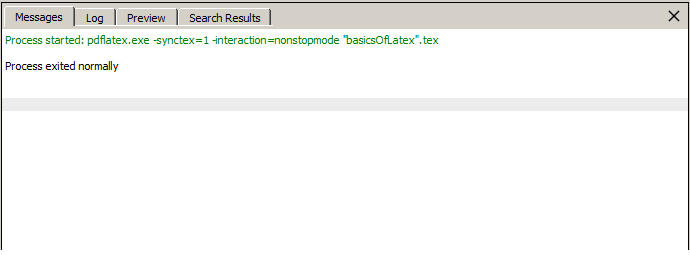
\includegraphics[height=1.2in]{basicsOfLatex/gettingStarted/texstudioConsole}
	\end{center}
While it is always good to fix the problem immediately (hit 
\includegraphics[height=0.25cm]{basicsOfLatex/gettingStarted/gotoError}), some errors can be ignored by hitting {\color{highlight}return} on the keyboard.
\end{frame}

\begin{frame} \frametitle{Errors are inevitable}
Errors are common in LaTeX. To help identify errors, it is recommended that you typeset frequently. Typeset every few sentences to verify your output matches what you anticipated. You can keep working while LaTeX processes your document. \\
\vspace{0.7cm}
Common errors that will make more sense as we go along...
\begin{itemize}
\item Misspelling a command
\item Not escaping special characters
\item Not balancing {\color{braces}\{}braces{\color{braces}\}}
\item Not balancing {\color{braces}\$}'s
\item Not balancing out beginning/ending environments (e.g. \texttt{\color{command}$\backslash$begin\color{braces}\{\color{black}document\color{braces}\}} and \texttt{\color{command}$\backslash$end\color{braces}\{\color{black}document\color{braces}\}})
\end{itemize}
\end{frame}

\begin{frame} \frametitle{Commenting}
Return to the basic file you just created. What's with all the red (or gray in Windows)? These are comments, which is writing that will be ignored by LaTeX. Comments are made by using the percent symbol: {\color{comment}\%}.
%\begin{tabbing} \small
%\hspace{1cm} \= text text text text text text text text text \\
%	\> text text text text text text text text text \\
%	\> {\color{comment}\% 929j(*\&@\#wfwj9f8uv9 ... this would be ignored} \\
%	\> {\color{comment}\% \hspace{0.5cm} even though it is atrocious and obnoxious} \\
%	\> text text text text text text text text text \\
%	\> text text text text text text text text text
%\end{tabbing}
\begin{center}
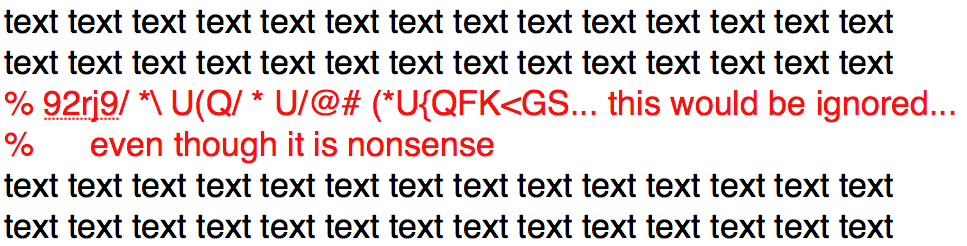
\includegraphics[height=0.6in]{basicsOfLatex/gettingStarted/commenting}
\end{center}
Any text following a {\color{comment}\%} on \emph{that line only} will be ignored by LaTeX.
\end{frame}

%text text text text text text text text text text text text text text text
%text text text text text text text text text text text text text text text
% 92rj9\*U(Q\*U\@\#\#(Wqej ... this would be ignored...
%       even though it is atrocious and obnoxious
%text text text text text text text text text text text text text text text
%text text text text text text text text text text text text text text text

\begin{frame} \frametitle{Navigation panel}
	
In TeXStudio has a very nice feature such as navigation panel.

\begin{center} 					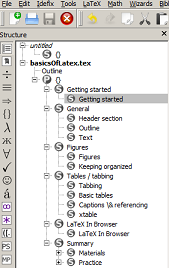
\includegraphics[height=5cm]{basicsOfLatex/gettingStarted/texstudioNavigationPanel}
\end{center}

This can be very useful when writing or editing a long document.
\end{frame}


\begin{frame} \frametitle{Example template}
	
Download the following zipped folder to your desktop
\begin{center}
	{\color{highlight} https://github.com/vdmitriyev/latex-intro/archive/master.zip}
\end{center}

Open template file {\color{highlight}latexTemp}. You can find mentioned file inside unziped folder under {LaTeX\_Basics/documents/latexTemp} path. 

\vspace{0.2cm}

Some notable contents:
\begin{itemize}
	\item Sample document ({\color{highlight}latexTemp.tex})
	\item PDF of this presentation
	\item {\color{highlight}figures} folder
	\item {\color{highlight}figures} folder
	\item UCLA thesis template files: {\color{highlight}uclathes-1.2} and {\color{highlight}uclathesUse}
\end{itemize}

{\color{highlight}latexTemp.tex} follows the most of this presentation and is filled with examples and extra comments. Open this file now.

\end{frame}


%%%%%%%%%%%%%%%%%%%%%%
%\part{}

\section[General]{General}

\subsection[Header section]{Header section}
\begin{frame} \frametitle{Document type}
The first command in every LaTeX document is the {\color{command}$\backslash$documentclass} command, which basically says what kind of document you are making.
\begin{center}

\includegraphics[height=0.2in]{basicsOfLatex/general/documentClass}
\end{center}
The default is the \texttt{\color{highlight}article} class.
\vspace{5mm}\\
Other classes: \texttt{\color{highlight}letter}, \texttt{\color{highlight}beamer} (presentations), \texttt{\color{highlight}book}. Examples and help can be found online for these other classes.
\vspace{5mm} \\
Alter \texttt{\color{highlight}[11pt]} to change the default font size for the document, if desired.
\end{frame}

\begin{frame} \frametitle{Packages}
Packages supply extra features and are generally free. They are always loaded at the start of the document. \\
\begin{figure}[htbp]
   \centering
   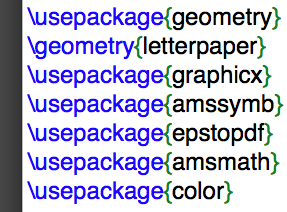
\includegraphics[height=0.7in]{basicsOfLatex/general/packages}
\end{figure}
Many common packages are included in a LaTeX installations, however, many other packages are not. Additional packages can be downloaded and installed, as needed.
\end{frame}

\subsection[Outline]{Outline}
\begin{frame} \frametitle{Sections and subsections}
Documents are often broken up into sections and subsections, and this hierarchy will automatically be numbered by LaTeX.
\begin{figure}[htbp]
   \centering
   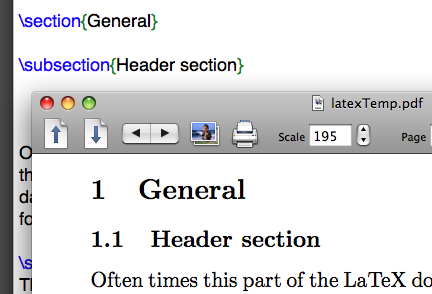
\includegraphics[height=1.4in]{basicsOfLatex/general/sectionsSubsections}
\end{figure}
\end{frame}

\subsection[Text]{Text}
\begin{frame} \frametitle{Paragraphs}
To end a paragraph and create a new one, do a double ``{\color{highlight}enter}'' and this creates a line break. \\
\vspace{0.5cm}
To put an extra line space between paragraphs, use the \texttt{\color{command}$\backslash\backslash$} command followed by a double line break in the \texttt{.tex} document.
\begin{figure}[htbp]
   \centering
   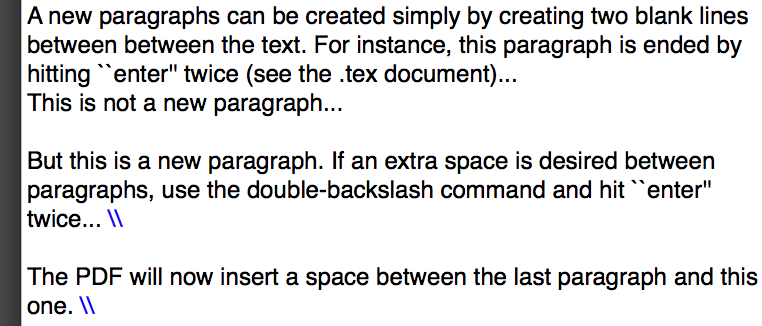
\includegraphics[height=1.4in]{basicsOfLatex/general/paragraphSpacing}
\end{figure}
\end{frame}

\begin{frame} \frametitle{Indentation and space}
{\bf Indentation. } To create an indent use \texttt{\color{command}$\backslash$indent}, and to prevent an indent use \texttt{\color{command}$\backslash$noindent}. Indenting can be suppressed via \texttt{\color{command}$\backslash$setlength}\texttt{\color{braces}\{}\texttt{\color{command}$\backslash$parindent}\texttt{\color{braces}\}}\texttt{\color{braces}\{}\texttt{0in}\texttt{\color{braces}\}}. \\
\vspace{0.7cm}
{\bf Space. } To create horizontal\hspace{1cm} space, use \texttt{\color{command}$\backslash$hspace}\texttt{\color{braces}\{}\texttt{1cm}\texttt{\color{braces}\}}. Similarly, use the \texttt{\color{command}$\backslash$vspace}\texttt{\color{braces}\{}\texttt{0.5cm}\texttt{\color{braces}\}} command, or to add extra space after a line break (more than the default), use \texttt{{\color{command}$\backslash\backslash$}[1cm]}. Negative distances may also be used. %\texttt{\color{command}$\backslash$hspace} and \texttt{\color{command}$\backslash$vspace} are generally more useful in tables than in text.
\end{frame}

\begin{frame} \frametitle{Playing with the font}
{\bf Emphasize (italicize). } Use the command \texttt{\color{command}$\backslash$emph}, e.g. \texttt{\color{command}$\backslash$emph}{\color{braces}\{}\texttt{emphasize\color{braces}\}}, to \emph{emphasize} (italicize) a single word. \\
\vspace{0.7cm}

{\bf More manipulation. } Text can also be \textbf{bolded} via \texttt{\color{command}$\backslash$textbf} or {\color{red} colored} via \texttt{\color{braces}$\{$\color{command}$\backslash$color\color{braces}$\{$\color{black}red\color{braces}$\}$\color{black}colored\color{braces}$\}$} (need package {\color{highlight}color}). Font can be made to look \texttt{typewriterish} via \texttt{\color{command}$\backslash$texttt}. \\
\vspace{0.7cm}

{\bf Font size. } Text can also be made {\tiny tiny}, {\scriptsize scriptsize}, {\footnotesize footnotesize}, {\small small}, {\large large}, {\Large Large}, {\LARGE LARGE}, etc. via \texttt{\color{command}$\backslash$tiny}, \texttt{\color{command}$\backslash$scriptsize}, etc.
\end{frame}

\begin{frame} \frametitle{Lists}
Lists can be created via
\begin{center}
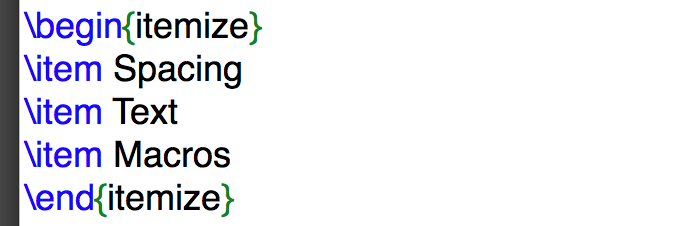
\includegraphics[height=0.7in]{basicsOfLatex/general/list}
\end{center}
which results in a bulleted list such as the following:
\begin{itemize}
\item Spacing
\item Text
\item Macros
\end{itemize}
A couple additional examples are in {\color{highlight}latexTemp.tex}.
\end{frame}

\begin{frame} \frametitle{Practice - 01}
Write two short paragraphs that includes a few words or phrases that have been \textit{italicized} and also some that have been \textbf{bolded}.

\vspace{7mm}

What should you do if you want a line break between the paragraphs? What if you only want the second paragraph indented?

\vspace{7mm}

Add the package {\color{highlight}color} and add color to some of your text. For instance, try 
\texttt{\color{braces}$\{$\color{command}$\backslash$color\color{braces}$\{$\color{black}red\color{braces}$\}$\color{black}Some text that will be colored red.\color{braces}$\}$}
\end{frame}


\section[Figures]{Figures}
\subsection[Figures]{Figures}
\begin{frame} \frametitle{Basic figures}
	Add figures using the {\color{command}$\backslash$includegraphics} command.
	\begin{center}
	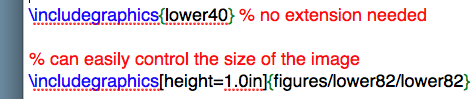
\includegraphics[height=15mm]{basicsOfLatex/figures/basicFigures}
	\end{center}
	The first file is stored in the same folder as the LaTeX file. The second is a couple folders away.
	\vspace{0.5cm} \\
	\emph{The files and folder names used should have no spaces.}
	\vspace{0.5cm} \\
	\texttt{[height=1.0in]} is an optional argument to control the figure size.
\end{frame}

\begin{frame} \frametitle{Figure centering}
	Just like tables, a figure can be centered:
	\begin{center}
	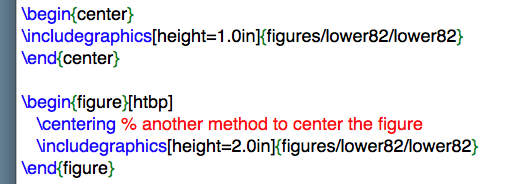
\includegraphics[height=1.1in]{basicsOfLatex/figures/centerFigure}
	\end{center}
	How does the second method look similar to the floating tables? (This is a floating figure.)
\end{frame}

\begin{frame} \frametitle{Adding a caption and referencing}
	Just like in the floating \texttt{\color{highlight}table} environment, a floating figure can have a caption and reference.
	\begin{center}
	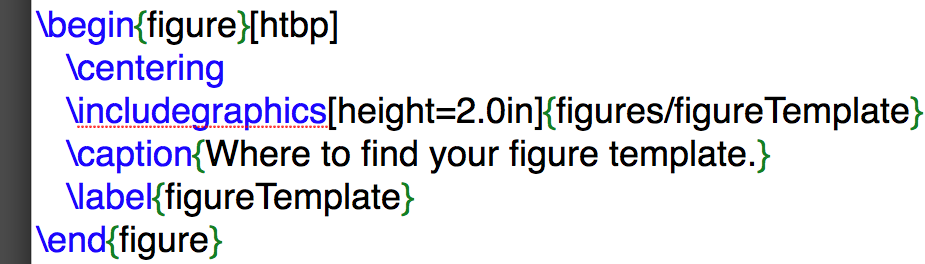
\includegraphics[height=0.9in]{basicsOfLatex/figures/figureWithCaptionLabel}
	\end{center}
	Just like with tables, the \texttt{\color{command}$\backslash$label} command must come after the \texttt{\color{command}$\backslash$caption} command for the reference to work properly.
	\vspace{5mm} \\
	Figure$\sim${\color{command}$\backslash$ref}{\color{braces}$\{${\color{black}figureTemplate}$\}$} is where to find your figure template.
\end{frame}

\subsection[Keeping organized]{Keeping organized}
\begin{frame} \frametitle{Keeping organized}
Some tips to keeping organized when using LaTeX:
	\begin{itemize}
		\item One LaTeX document per folder.
		\item When choosing a \texttt{\color{command}$\backslash$label} name for a figure, have it match the figure file name.
		\item Organize figure files into folders.
		\item If you use code to produce a figure, save it to the same folder as the figure and with the same name (but a different extension, of course).
		\item Remember, no spaces in file or folder names.
	\end{itemize}
\end{frame}

\begin{frame}	\frametitle{Practice - 02}
	
	Using the image in \texttt{\color{highlight}latexTemp/figures/lower82/}, produce the following plot. Make it 0.8 inches tall, center it, add a caption, and add a reference. Be sure to write a sentence that references the Figure and compile your LaTeX document twice so the reference works. \\
	
		\begin{center}
			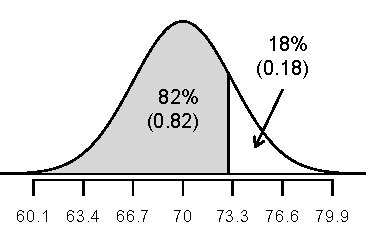
\includegraphics[height=1.3in]{documents/latexTemp/figures/lower82/lower82}
		\end{center}
		
	Feel free to utilize examples in \texttt{\color{highlight}latexTemp.tex} or to use the LaTeX Float Figure template.
		
\end{frame}


\section[Tables / tabbing]{Tables / tabbing}

\subsection[Tabbing]{Tabbing}
\begin{frame} \frametitle{Tabbing}
	Like in other text editors, LaTeX offers tabbing. While this environment tends to rarely be used, it can be very useful under particular conditions.
	\begin{figure}[htbp]
		\centering
		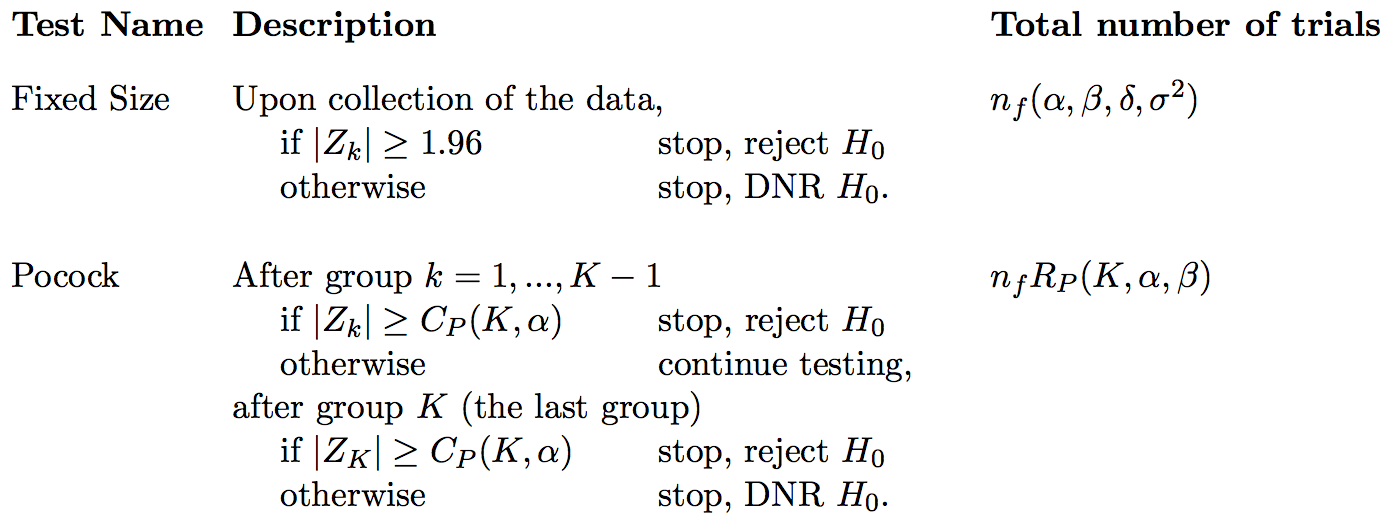
\includegraphics[height=1.3in]{basicsOfLatex/tabTable/tabbingExample}
	\end{figure}
	See {\color{highlight}latexTemp.tex} for a brief introduction to tabbing and a few examples.
\end{frame}

\subsection[Basic tables]{Basic tables}
\begin{frame} \frametitle{Basic tables}
	Tables are created using the \texttt{\color{highlight}tabular} environment. The \text{\color{braces}\{}\texttt{lcr}\texttt{\color{braces}\}} gives the alignment. The ampersands ({\color{highlight}\&}) are used to define when to go to the next column.
	\begin{figure}[htbp]
		\centering
		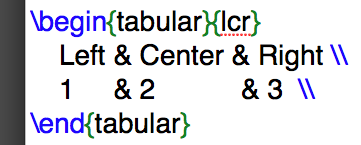
\includegraphics[height=0.55in]{basicsOfLatex/tabTable/basicTable}
	\end{figure}
	The \texttt{\color{command}$\backslash\backslash$} command tells LaTeX to start a new row.  \\
	\vspace{0.3cm}
	The result: \\
	\vspace{0.3cm}
	\begin{tabular}{lcr} % lcr means make the 1st column left aligned, the 2nd centered, and the 3rd right aligned
		Left & Center & Right \\ % the amperstands (&) define where to start the next column
		1     & 2           & 3  \\
	\end{tabular}
\end{frame}

\begin{frame} \frametitle{Centering and adding lines}
	Building the table up:
	\begin{figure}[htbp]
		\centering
		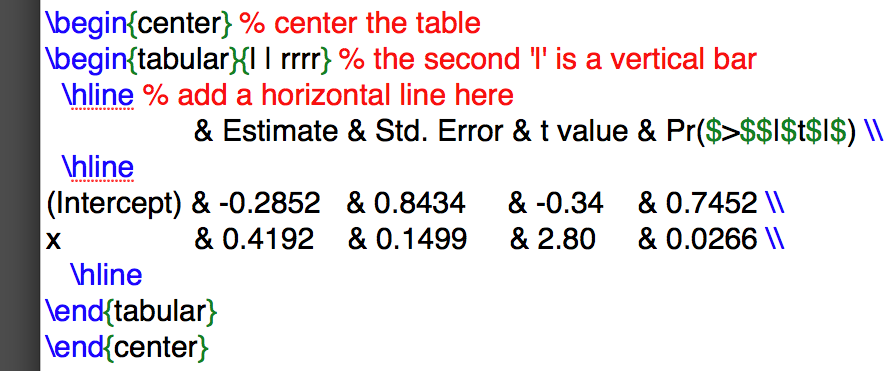
\includegraphics[height=1.0in]{basicsOfLatex/tabTable/centeredTable}
	\end{figure}
	The result: \\
	\vspace{0.3cm}
	\begin{center} % center the table
		\begin{tabular}{l | rrrr} % the second 'l' is a vertical bar
			\hline % add a horizontal line here
			& Estimate & Std. Error & t value & Pr($>$$|$t$|$) \\
			\hline
			(Intercept) & -0.2852   & 0.8434     & -0.34    & 0.7452 \\
			x                & 0.4192    & 0.1499     & 2.80     & 0.0266 \\
			\hline
		\end{tabular}
	\end{center}
\end{frame}

\subsection[Captions \& referencing]{Captions \& referencing}
\begin{frame} \frametitle{Floating table with a caption}
	To add a caption or label, the table must be \emph{floated} (i.e. add on the \texttt{\color{highlight}table} environment). Then \texttt{\color{command}$\backslash$caption} can be used:
	\begin{figure}[htbp]
		\centering
		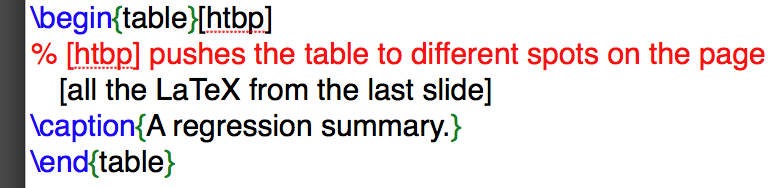
\includegraphics[height=0.6in]{basicsOfLatex/tabTable/floatTable}
	\end{figure}
	The output:
	\begin{table}[htbp]
		\begin{center} % center the table
			\begin{tabular}{l | rrrr} % the second 'l' is a vertical bar
				\hline % add a horizontal line here
				& Estimate & Std. Error & t value & Pr($>$$|$t$|$) \\
				\hline
				(Intercept) & -0.2852   & 0.8434     & -0.34    & 0.7452 \\
				x                & 0.4192    & 0.1499     & 2.80     & 0.0266 \\
				\hline
			\end{tabular}
		\end{center}
		\caption{A regression summary.}
	\end{table}
	The table is numbered when a caption is added in the \texttt{\color{highlight}article} document class.
\end{frame}

\begin{frame} \frametitle{Referencing}
	%Tables can be dynamically referenced (many examples in {\color{highlight}latexTemp.tex}).
	%\vspace{5mm} \\
	Suppose we are writing a document and refer to Table 4 in our text. Two days later, we decide to add another table earlier in the document. Now Table 4 is actually Table 5 and we need to change all the 4s to 5s (and 5s to 6s, and so on).
	\vspace{5mm} \\
	Instead, we tag each table with a unique label. We reference the label, not the number.
	\begin{figure}[htbp]
		\centering
		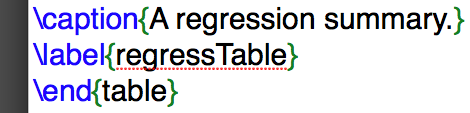
\includegraphics[height=0.4in]{basicsOfLatex/tabTable/labelTable}
	\end{figure}
	\texttt{\color{command}$\backslash$label}\texttt{\color{braces}\{}\texttt{regressTable}\texttt{\color{braces}\}} labels the table and then this table can be referenced using the LaTeX code \texttt{Table$\sim$}\texttt{\color{command}$\backslash$ref}\texttt{\color{braces}\{}\texttt{regressTable}\texttt{\color{braces}\}}.
\end{frame}

\subsection[xtable]{xtable}
\begin{frame} \frametitle{Using the R package \texttt{xtable}} 
	Inside R: \\
	\vspace{0.3cm} \small
	\hspace{0.3cm}\texttt{> library(xtable) \# may need install.packages('xtable')} \\
	\hspace{0.3cm}\texttt{> x <- 1:9} \\
	\hspace{0.3cm}\texttt{> z <- rnorm(9)} \\
	\hspace{0.3cm}\texttt{> y <- x$/$7 + z$^*$2 + rnorm(9)} \\
	\hspace{0.3cm}\texttt{> xtable(summary(lm(y $\sim$ x$+$z)))} \\
	\hspace{0.3cm}\texttt{... output that can be copied/pasted into LaTeX ...} \\
	\vspace{0.3cm} \normalsize
	R output directly copied/pasted into LaTeX:
	\begin{table}[ht]
		\begin{center}
			\begin{tabular}{rrrrr}
				\hline
				& Estimate & Std. Error & t value & Pr($>$$|$t$|$) \\
				\hline
				(Intercept) & -0.1563 & 0.6243 & -0.25 & 0.8107 \\
				x & 0.1094 & 0.1145 & 0.96 & 0.3760 \\
				z & 2.6170 & 0.4308 & 6.08 & 0.0009 \\
				\hline
			\end{tabular}
		\end{center}
	\end{table}
\end{frame}

\begin{frame} \frametitle{Practice - 03}
	
	Produce the following result:
	\begin{center}
		\begin{tabular}{l rrr}
			\hline
			& mean & sd & n \\
			\hline
			S1 & 6.5 & 1.3 & 17 \\
			S2 & 12.2 & 1.4 & 25 \\
			\hline
		\end{tabular}
	\end{center}
	
	Some examples may be utilized in \texttt{\color{highlight}latexTemp.tex}.
	
\end{frame}


\section[LaTeX In Browser]{LaTeX In Browser}
\subsection{LaTeX In Browser}
	
	\begin{frame} \frametitle{Usage LaTeX in Browser}
		Besides using LaTeX on desktops, there is a great possibility to bring the same experience into browsers. Benefits of using LaTeX (especially math/equation part) directly inside browsers is hard to overestimate.
	\end{frame}
	
	\begin{frame} \frametitle{LaTeX in Web - Tools}
		Number of software tools and libraries are available to deal with LaTeX directly in browser.\\
		
		\begin{itemize}
			\item \href{https://www.mathjax.org/}{MathJax} - Most popular JavaScript library
			\item \href{https://khan.github.io/KaTeX/}{KaTeX} - JavaScript library from Khan Academy
			\item ...
		\end{itemize}
	
	\end{frame}
	
		\begin{frame} \frametitle{LaTeX in Web - Examples}
			
			\begin{itemize}
				\item \href{http://www.papeeria.com/}{papeeria - Online LaTeX Editor (Free and easy)}
				\item \href{http://arachnoid.com/latex/}{Interactive LaTeX Editor}
				\item \href{https://github.com/mathjax/MathJax/blob/master/test/sample-dynamic-2.html}{MathJax Live Demo}
				\item \href{https://ipython.org/ipython-doc/3/install/install.html\#mathjax}{Jupyter Notebook (former IPython)}
			\end{itemize}
			
		\end{frame}

\section[Summary]{Summary}

%\subsection[Examples]{Examples}
%\frame{ \frametitle{Diverse possibilities}
%LaTeX has a lot of power to do diverse tasks:
%\begin{itemize}
%\item Chemistry figures
%\item Circuits
%\item Feynman diagrams
%\item Musical scores
%\item Crossword puzzles
%\item Sudoku puzzles
%\end{itemize}
%These different applications require packages that are generally not included in a basic download of LaTeX but that can typically be downloaded at no cost. \\
%\vspace{0.3cm}
%The ability to make elegant documents and figures is one of LaTeX's major draws. It offers users nearly unlimited control of their documents (even though it might feel a bit out of control at first).
%}

\subsection[Materials]{Materials}
\begin{frame} 
		\frametitle{Materials}

		Tools
		\begin{itemize}
			\item \href{http://www.tablesgenerator.com/latex_tables}{LaTeX Tables Generator}
			\item \href{http://truben.no/table/}{LaTeX Table Editor}
			\item \href{http://truben.no/latex/bibtex/}{BibTeX Editor}
		\end{itemize}
		
		Books, Articles
		\begin{itemize}
			\item \emph{Guide to LaTeX}, by Helmut Kopka and Patrick W. Daly
			\item \href{http://mirror.physik-pool.tu-berlin.de/tex-archive/info/first-latex-doc/first-latex-doc.pdf}{Getting something out of LATEX}, by Jim Hef­feron
		\end{itemize}				
		
		Online materials
		\begin{itemize}
			\item \href{http://www.latex-tutorial.com/tutorials/beginners/}{Tutorial for "Beginners"}
			\item \href{http://www.math.uiuc.edu/~hildebr/tex/latex-start.html}{Getting Started with LaTeX}
			\item \href{https://www.tug.org/begin.html}{Getting Started with TeX, LaTeX, and Friends}
			\item \href{http://www.andy-roberts.net/writing/latexl}{Getting to Grips with LaTeX}
			\item \href{http://wch.github.io/latexsheet/}{LaTeX cheat sheet}
		\end{itemize}				
		
\end{frame}

\subsection[Practice]{Practice}
\begin{frame}
		\frametitle{Practice - Summary}

		Write a 2 page document in LaTeX (or transfer another document not in LaTeX into LaTeX).
		\vspace{0.5cm}
		
		Your document must include following artifacts:\\
		\begin{itemize}
			\item 2 or more sections with at least one subsection
			\item couple of paragraphs 
			\item at least one figure
			\item at least one table
			\item text references using {\color{command}$\backslash$label}s to the figure and table
		\end{itemize}
	
\end{frame}


\end{document}